\documentclass[12pt, oneside]{article}   	% use "amsart" instead of "article" for AMSLaTeX format
\usepackage{geometry}                		% See geometry.pdf to learn the layout options. There are lots.
\geometry{a4paper, total={6.8in, 8.5in}}
\usepackage{fancyhdr}
\usepackage{amsmath}
\usepackage{amssymb}
\usepackage{graphicx}				% Use pdf, png, jpg, or eps§ with pdflatex; use eps in DVI mode
\graphicspath{ {./} }

\begin{document}
\pagestyle{fancy}
\fancyhead{}
\fancyhead[LO]{\textbf{CSE 5370}\\\textbf{BIO INFORMATICS}}
\fancyhead[RO]{\textbf{Sanjana Reddy Thigulla}\\1002142811}
\fancyhead[CO]{\LARGE{\textbf{Homework-1}}}

\begin{enumerate}
\item Executing the given “datasetGenerator.py” script on terminal with the UTA ID: 1002142811 has generated a unique dataset with name 1002142811.csv. It is included in the zip file.

\item 

\begin{itemize}
\item The fisher’s exact test is a statistical test performed on the contingency tables and tests whether the odds ratio of the underlying populations are close to 1 or not

\item The odds ratio is defined as the ratio of the odds of event $A$ in the presence of $B$ and the odds of $A$ in the absence of $B$. it quantifies the strength of the association between two events.

\item Oddsratio and $p$ value have been calculated using fisher exact function from scipy module.

\item Null hypothesis: $C$-allele or $T$-allele SNPs don’t contribute to person’s risk of developing the complex trait. (independent)

\item Alternative hypothesis: $C$-allele or $T$-allele SNPs contribute to person’s risk of developing the complex trait. (dependent)

\item The fisher exact function takes 2 inputs, the $2\times2$ matrix/table and alternative. By default alternative is two-sided that is the odds ratio is not one. 

\item The total number of significant $p$ values is 299.

\item The fisher exact function gives 2 values, oddsratio and $p$-value. This p-value is then compared with effective p-value to find out whether the SNP is significant.


\end{itemize}

\item The assumed $p$-value is $5 \times 10^{-8}$ . Bonferroni corrected p-value is given by

\begin{align*}
&= \frac{(\text{original } p \text{ value})}{(\text{no of tests performed})}\\
&= \frac{5 \times 10^{-8}}{1000}\\
&= 5 \times 10^{-11}
\end{align*}

Therefore, the Bonferroni corrected p-value is $5 \times 10^{-11}$.

After Bonferroni correction, Total number of new significant $p$ values is 209.

The \emph{results.csv} file depicts the results of the fisher exact test after comparing with the  effective $p$ value and corrected pvalue.

\item Using the negative logarithm of (p value) a pseudo Manhattan plot (Figure \ref{fig:mesh1}) has been generated.

\begin{itemize}
\item This plot depicts the SNPs and their p values; all of the significant SNPs over the threshold indicate that the C alleles will have an impact on the complex phenotype.

\item The upper red line represents the standard p-value threshold, and the lower redline represents the Bonferroni-corrected threshold value.
\end{itemize}

\newpage
\thispagestyle{empty}

\begin{figure}[!h]
\centering
\begin{minipage}[c]{1\textwidth}
    \centering
    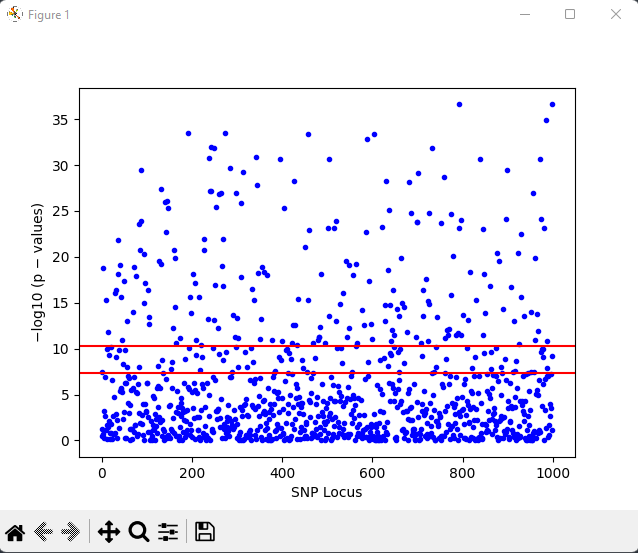
\includegraphics[width=0.8\textwidth]{image1}
    \caption{\footnotesize{Pseudo Manhattan plot}}
    \label{fig:mesh1}
\end{minipage}
\end{figure}

\end{enumerate}
\end{document}